% !TEX root = main21.tex
\section{A wider-grid GROMM v1 calibration and VIX}
\label{sec:wide-grid}
% Generated from completed reports; see metrics.json.
\newcommand{\WideVixMaeReduction}{75.33}
\newcommand{\WideCoreCoverage}{97.299}
\newcommand{\WideExplainedVariance}{75.87}
\newcommand{\WideOverallConditionalMedian}{1.98624}
\newcommand{\WideOverallMidpointMae}{0.56549}
\newcommand{\WideSquaredMean}{1.311}
\newcommand{\WideSquaredSe}{1.317}
\newcommand{\WideSquaredCiLow}{-1.270}
\newcommand{\WideSquaredCiHigh}{3.892}
\newcommand{\WideEntropyMean}{1.312}
\newcommand{\WideEntropySe}{1.318}
\newcommand{\WideEntropyCiLow}{-1.272}
\newcommand{\WideEntropyCiHigh}{3.896}


We consider a separately calibrated extension of the original GROMM v1,
\texttt{Gromm-v1-4,3}, intended
to improve coverage of the option wings relevant to variance swaps and VIX.
It has the same SDLV architecture: 25 daily expiries, 200 interior strikes,
5,000 direct state coordinates per date, and an independent 5\% Black
smoothing factor. Both the 100-node one-day template and the 100-node
25-day template are widened to NMS $[-4,3]$; the one-day grid is retained.
NMS denotes the main paper's regularized, ATM-volatility-scaled
log-moneyness coordinate; the original templates span $[-2.5,1.5]$.
The templates are merged into a common support as before. This changes the
strike coverage, not the model's 25-business-day maturity limit.
With the interior-node count held fixed, the wider support redistributes
strike resolution rather than adding state coordinates.

\subsection{Fresh calibration and market fit}

The new fit uses the same 891 dates, 3 January 2022--29 August 2025, and the
same upstream market-quality filters, but removes the final NMS quote cutoff.
All 3,141,110 remaining call and put intervals are used. Quotes with their
own expiry-specific NMS in $[-3.5,2.5]$ receive weight one; all others receive
weight $0.1$. This is not a claim to retain every raw exchange quote. Each
day's weighted loss is normalized by its sum of quote weights, and the
objective averages equally across days. The loss remains bid--ask excess
plus $0.05$ times absolute midpoint error, in half-spread units, together
with the original DLV cap penalty.

All daily model states were fitted from an ATM initializer, without
transferring the original trained weights. The complete original schedule
was run: 300 Adam epochs with cosine learning rate $0.02\to0.001$, followed
by 700 epochs with $0.005\to0.00005$, resetting Adam at the continuation
boundary. No VIX observations entered this objective.

\begin{table}[H]
\centering\small
\begin{tabular}{lrrrr}
\toprule
Fit / quote subset & Quotes & \% excess & Mean excess & Cond. mean \\
\midrule
Original v1, original range & 2,192,458 & 2.679\% & 0.03450 & 1.28797 \\
Wider fit, original range & 2,192,458 & 2.636\% & 0.03435 & 1.30311 \\
Wider fit, core & 2,465,684 & 2.701\% & 0.03484 & 1.28996 \\
Wider fit, wings & 675,426 & 31.635\% & 1.31125 & 4.14489 \\
Wider fit, all quotes & 3,141,110 & 8.923\% & 0.30930 & 3.46650 \\
Wider fit, 29 Aug. (all) & 4,190 & 15.012\% & 0.62411 & 4.15740 \\
\bottomrule
\end{tabular}
\caption{Static-fit errors beyond the bid--ask interval, in half-spread units. All statistics are unweighted quote-level summaries, not the weighted training objective. Conditional means include only quotes with positive excess. The original-range rows cover the same 2,192,458 retained quotes; the final row is a separate single-date summary.}
\label{tab:wide-static-fit}
\end{table}


Table~\ref{tab:wide-static-fit} separates the expanded quote universe from
the original comparison set. The wider fit covers \WideCoreCoverage\% of
the core quotes, whereas the downweighted wings remain appreciably harder
to fit. Across the full expanded universe, the conditional median excess
is \WideOverallConditionalMedian{} half-spreads and midpoint MAE is
\WideOverallMidpointMae{} half-spreads. The original-range rows should be
used when comparing static fit with the original GROMM v1;
the all-quote and single-date rows have different denominators.
Because grid coverage, quote scope and loss weights change together,
this experiment does not isolate the effect of grid width alone.

\subsection{Fresh diffusion estimation and risk-neutral audit}

The diffusion is re-estimated from the new historical fitted surfaces,
not transferred from GROMM v1. The estimator uses 710 exact one-session
pairs ending no later than 31 December 2024, with the same fixed-contract
alignment and Gaussian smoothing widths of one expiry and two strike nodes.
The eight-factor system, including the front-spot factor, captures
\WideExplainedVariance\% of the smoothed innovation variance. Thus the
29 August 2025 initial state is contemporaneously calibrated, while the
diffusion-estimation window ends before that date.
Appendix~\ref{app:wide-grid-factors} shows the new mean implied-volatility
surface, the saved innovation spectrum and all eight retained factor responses.

We use the same front-density bridge and recomputed risk-neutral DLV drift
as in the original model, with eight uniform substeps per day. From the
completed new state we generate 100,000 fresh paths arranged as 50,000
independent antithetic pairs. The 20-business-day trading universe is spot
plus 44 options, constructed from the new initial surface with the same
NMS and maturity rule as the main paper: eleven initially OTM calls or puts
at each of 5, 10, 15 and 20 business days, with cash strikes fixed thereafter.
Appendix~\ref{sec:wide-audit-definition} defines the reported statistics.
Both conditional policies are trained afresh, with whole paths and complete
pairs kept together in each fold. No old diffusion factors, simulated
populations or trained conditional policies are reused.

\begin{table}[H]
\centering\small
\begin{tabular}{rrrrrrr}
\toprule
$N$ & Max. $|z|$ & 99\% $|z|$ & $N_{2.576}$ & $N_5$ & $T_{\rm sqr}$ & $T_{\rm ent}$ \\
\midrule
570 & 2.426 & 2.118 & 0 & 0 & 0.995 & 0.995 \\
\bottomrule
\end{tabular}
\caption{Fresh GROMM v1-4,3 restricted-universe $\Q$ audit: 100,000 paths, 50,000 antithetic pairs, 20 business days, spot plus 44 options; eight factors and eight steps per day. The statistics and colour conventions are those of Appendix~\ref{sec:wide-audit-definition}.}
\label{tab:wide-q-audit}
\end{table}


None of the 570 day--instrument coordinates exceeds $2.576$ standard errors.
The squared policy's out-of-fold mean and pair-based standard error are
$(\WideSquaredMean,\WideSquaredSe)\times10^{-9}$ daily spot units, with 95\%
interval $[\WideSquaredCiLow,\WideSquaredCiHigh]\times10^{-9}$.
For the entropy policy the corresponding values are
$(\WideEntropyMean,\WideEntropySe)\times10^{-9}$ and
$[\WideEntropyCiLow,\WideEntropyCiHigh]\times10^{-9}$.
Both intervals contain zero. These diagnostics are consistent with the
risk-neutral null for the tested instrument universe and policy class;
they are not a proof over all strategies. In particular, the wider model
has \emph{not} undergone the main paper's 25-day full-instrument-grid audit,
nor a separate test of every
new wing strike. No new physical-measure simulation audit is claimed here.

\subsection{Historical VIX comparison}

Figure~\ref{fig:wide-vix-comparison} compares the original and wider models
with the official Cboe closing VIX and a reconstruction from the filtered
market spreads supplied to SANOS. The discrete model series reprice the
same market-selected option strips, with observed bid cutoffs and the
same expiry interpolation. The analytic series instead use the model's
full-strike log-contract variance at those same two expiries.
Appendix~\ref{app:wide-grid-details} specifies the formulas and clocks.

\begin{figure}[H]
  \centering
  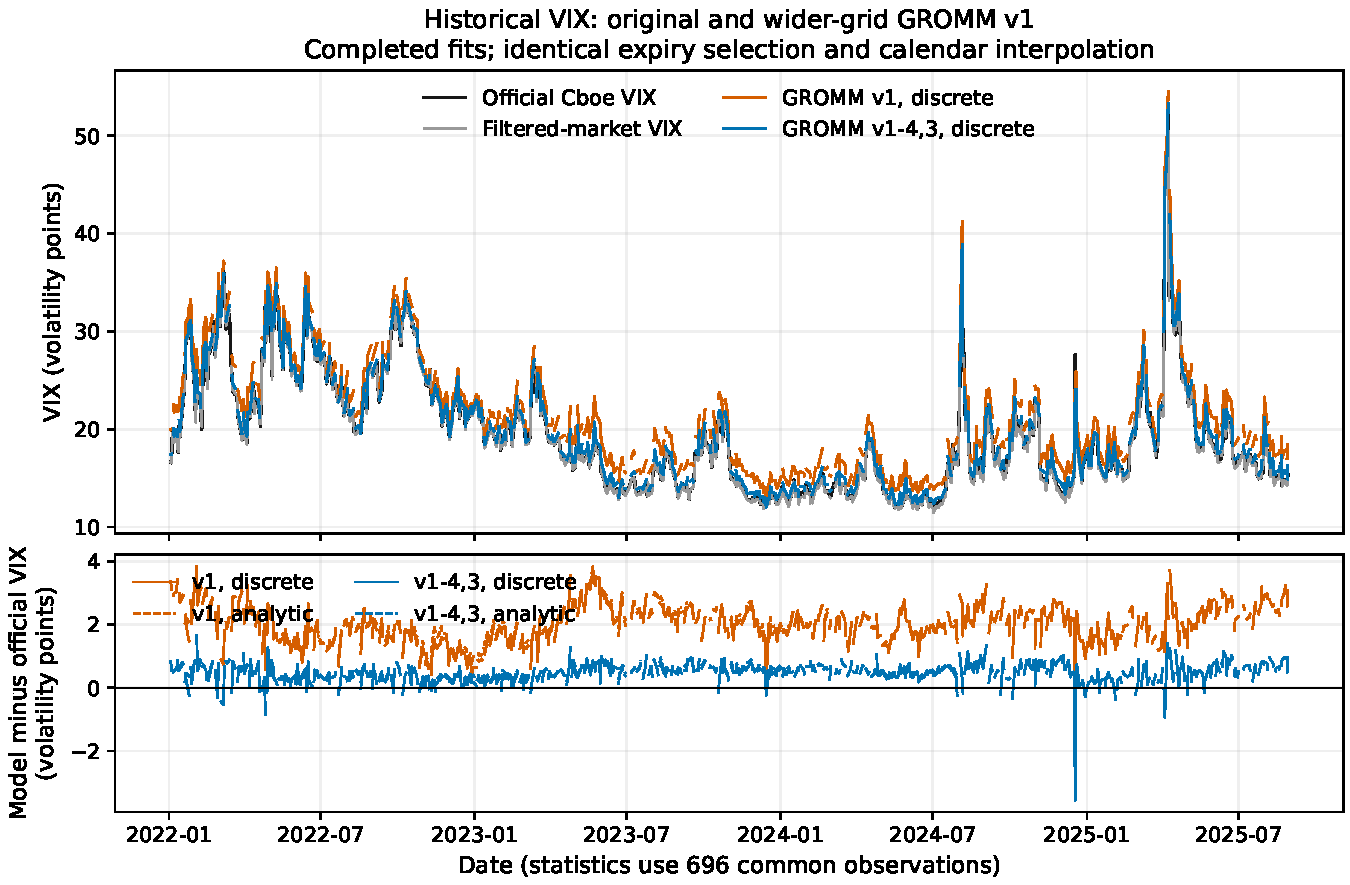
\includegraphics[width=\textwidth]{generated/wide_grid/gromm_v1_wide_vix.pdf}
  \caption{Historical VIX levels (top) and model errors relative to the
  official close (bottom). Orange denotes the original GROMM v1 and blue
  the completed GROMM v1-4,3 calibration. Solid model curves use the
  market-selected discrete strip; dashed error curves use the analytic
  full-strike variance swap. The grey top curve uses filtered market input
  spreads, not fitted SANOS prices. Statistics use the same 696 complete
  dates; missing model maturities are not extrapolated or filled in.}
  \label{fig:wide-vix-comparison}
\end{figure}

\begin{table}[H]
\centering\small
\begin{tabular}{lrrrrr}
\toprule
Series & Bias & MAE & RMSE & Corr. & 29 Aug. \\
\midrule
Raw-market strip & +0.028 & 0.142 & 0.265 & 0.99903 & 15.405 \\
Filtered SANOS input & -0.181 & 0.235 & 0.349 & 0.99873 & 15.197 \\
GROMM v1, discrete & +1.999 & 2.005 & 2.094 & 0.99446 & 18.434 \\
GROMM v1, analytic & +2.062 & 2.068 & 2.149 & 0.99481 & 18.432 \\
GROMM v1-4,3, discrete & +0.461 & 0.495 & 0.568 & 0.99848 & 16.314 \\
GROMM v1-4,3, analytic & +0.497 & 0.528 & 0.595 & 0.99853 & 16.318 \\
\bottomrule
\end{tabular}
\caption{Historical VIX comparison on the same 696 complete dates. Errors and the reference-date levels are in volatility percentage points; the benchmark is the official Cboe close (15.360 on 29 August 2025). Analytic values use the full-strike log contract at the same two expiries and the same calendar interpolation as the discrete strip, not direct evaluation at a different 30-day business maturity.}
\label{tab:wide-vix}
\end{table}


Discrete VIX MAE falls from 2.005 to 0.495 volatility points, a
\WideVixMaeReduction\% reduction on identical dates. The wider model's
analytic series has MAE 0.528 and RMSE 0.595; its remaining positive bias
shows that the wider calibration does not fully remove the discrepancy.
On the reference date the official close is 15.360, compared with 18.434
for the original discrete model and 16.314 for the wider discrete model.

There are 696 common model observations out of 891 fitted dates: on 186
dates a required Friday maturity exceeds the 25-business-day horizon, and
nine dates lack an eligible expiry bracket. The raw-market and filtered-input
reconstructions have 882 observations individually; Table~\ref{tab:wide-vix}
restricts them to the same 696 dates as the models. This is a historical
comparison of contemporaneously calibrated surfaces, not an out-of-sample
VIX forecast or a fit to VIX. Although the implemented discrete formula
follows the Cboe strike-selection and interpolation rules, archived
OptionMetrics end-of-day quotes and zero curves do not reproduce Cboe's
synchronous inputs and intraday filtering. We therefore do not claim an
exact reconstruction of the published closing tick.
